\documentclass{beamer}
    \usepackage[utf8]{inputenc}
    
    \usetheme{Madrid}
    \usecolortheme{default}
    \usepackage{amsmath,amssymb,amsfonts,amsthm}
    \usepackage{mathtools}
    \usepackage{txfonts}
    \usepackage{tkz-euclide}
    \usepackage{listings}
    \usepackage{adjustbox}
    \usepackage{array}
    \usepackage{gensymb}
    \usepackage{tabularx}
    \usepackage{gvv}
    \usepackage{lmodern}
    \usepackage{circuitikz}
    \usepackage{tikz}
    \lstset{literate={·}{{$\cdot$}}1 {λ}{{$\lambda$}}1 {→}{{$\to$}}1}
    \usepackage{graphicx}
    
    \setbeamertemplate{page number in head/foot}[totalframenumber]
    
    \usepackage{tcolorbox}
    \tcbuselibrary{minted,breakable,xparse,skins}
    
    
    
    \definecolor{bg}{gray}{0.95}
    \DeclareTCBListing{mintedbox}{O{}m!O{}}{%
      breakable=true,
      listing engine=minted,
      listing only,
      minted language=#2,
      minted style=default,
      minted options={%
        linenos,
        gobble=0,
        breaklines=true,
        breakafter=,,
        fontsize=\small,
        numbersep=8pt,
        #1},
      boxsep=0pt,
      left skip=0pt,
      right skip=0pt,
      left=25pt,
      right=0pt,
      top=3pt,
      bottom=3pt,
      arc=5pt,
      leftrule=0pt,
      rightrule=0pt,
      bottomrule=2pt,
      toprule=2pt,
      colback=bg,
      colframe=orange!70,
      enhanced,
      overlay={%
        \begin{tcbclipinterior}
        \fill[orange!20!white] (frame.south west) rectangle ([xshift=20pt]frame.north west);
        \end{tcbclipinterior}},
      #3,
    }
    \lstset{
        language=C,
        basicstyle=\ttfamily\small,
        keywordstyle=\color{blue},
        stringstyle=\color{orange},
        commentstyle=\color{green!60!black},
        numbers=left,
        numberstyle=\tiny\color{gray},
        breaklines=true,
        showstringspaces=false,
    }
    %------------------------------------------------------------
    %This block of code defines the information to appear in the
    %Title page
    \title %optional
    {12.353}
    \date{11 October, 2025}
    %\subtitle{A short story}
    
    \author % (optional)
    {INDHIRESH S - EE25BTECH11027}
    
    \begin{document}
    
    \frame{\titlepage}
    
    \begin{frame}{Question}
   Which one of the following describes the relationship among the three vectors
\begin{align*}
    \hat{i}+\hat{k}+\hat{k},2\hat{i}+3\hat{j}+\hat{k},5\hat{i}+6\hat{j}+4\hat{k}
\end{align*}
\begin{enumerate}
    \item The vectors are mutually perpendicular
    \item The vectors are linearly dependent
    \item The vectors are linearly independent
    \item The vectors are unit vectors
\end{enumerate}
    \end{frame}
    
    \begin{frame}[allowframebreaks] 
    \frametitle{Equation}
        \centering
        \label{tab:parameters}
Let
\begin{align}
\Vec{A}=\myvec{1\\1\\1}\;\;\Vec{B}=\myvec{2\\3\\1}\;\;and\;\;\myvec{5\\6\\4}
\end{align}
Let 
\begin{align}
   \Vec{M}=\myvec{\Vec{A}&\Vec{B}&\Vec{C}}
\end{align}

\begin{align}
    \Vec{M}=\myvec{1&2&5\\1&3&6\\1&1&4}
\end{align}


    \end{frame}
    
    \begin{frame}
    \frametitle{Theoretical Solution}
  Now applying row operations\\
$R_2\longrightarrow R_2-R_1$ and \\
$R_3\longrightarrow R_3-R_1$
\begin{align}
   \myvec{1&2&5\\1&3&6\\1&1&4}=\myvec{1&2&5\\0&1&1\\0&-1&-1}
\end{align}



    \end{frame}
    
    \begin{frame}
    \frametitle{Theoretical solution}
 Now doing row operation\\
$R_3\longrightarrow R_3+R_2$
\begin{align}
   \myvec{1&2&5\\0&1&1\\0&-1&-1}= \myvec{1&2&5\\0&1&1\\0&0&0}
\end{align}
Here the rank of the matrix is 2.\\
Since the rank is less than the number of vectors , the vectors are linearly dependent




    \end{frame}


    
   
    \begin{frame}[fragile]
        \frametitle{C Code}
        \begin{lstlisting}
#include <math.h>

#define N 3
#define TOLERANCE 1e-9

int check_vectors(double v1[], double v2[], double v3[]) {
    double mat[N][N];
    
    // Create a matrix from the input vectors (as columns)
    for (int i = 0; i < N; i++) {
        mat[i][0] = v1[i];
        mat[i][1] = v2[i];
        mat[i][2] = v3[i];
    }
    
   
        \end{lstlisting}
    \end{frame}
    
    \begin{frame}[fragile]
        \frametitle{C Code}
        \begin{lstlisting}
    // --- Gaussian Elimination to find rank ---
    for (int col = 0; col < N; col++) {
        int pivot_row = col;
        for (int i = col + 1; i < N; i++) {
            if (fabs(mat[i][col]) > fabs(mat[pivot_row][col])) {
                pivot_row = i;
            }
        }
        
        if (pivot_row != col) {
            for (int i = 0; i < N; i++) {
                double temp = mat[col][i];
                mat[col][i] = mat[pivot_row][i];
                mat[pivot_row][i] = temp;
            }
        }

        
        \end{lstlisting}
    \end{frame}

    \begin{frame}[fragile]
        \frametitle{C Code}
        \begin{lstlisting}
   if (fabs(mat[col][col]) < TOLERANCE) continue;

        for (int i = 0; i < N; i++) {
            if (i != col) {
                double factor = mat[i][col] / mat[col][col];
                for (int j = col; j < N; j++) {
                    mat[i][j] -= factor * mat[col][j];
                }
            }
        }
    }

    int zero_rows = 0;
    for (int i = 0; i < N; i++) {
        int all_zeros = 1;
        for (int j = 0; j < N; j++) {
            if (fabs(mat[i][j]) > TOLERANCE) {
                all_zeros = 0;
              
            
        \end{lstlisting}
    \end{frame}
    \begin{frame}[fragile]
        \frametitle{C Code}
        \begin{lstlisting}

          break;
  }
        }
        if (all_zeros) zero_rows++;
    }
    
    int rank = N - zero_rows;
    
    return (rank < 3) ? 2 : 3;
}
        \end{lstlisting}
    \end{frame}
    
   
    
    \begin{frame}[fragile]
        \frametitle{Python Code}
        \begin{lstlisting}
import ctypes
import os
import platform
import numpy as np
import matplotlib.pyplot as plt
from mpl_toolkits.mplot3d import Axes3D

# --- Function to get vector input from the user ---
def get_vector_from_user(vector_name: str) -> list[float]:
    """Prompts the user for 3 vector components and returns them as a list."""
    while True:
        try:
            input_str = input(f"Enter the 3 components for vector {vector_name} (e.g., 1, 2, 3): ")
            components = [float(item) for item in input_str.split(',')]
            


        \end{lstlisting}
    \end{frame}
    
    \begin{frame}[fragile]
        \frametitle{Python Code}
        \begin{lstlisting}
 if len(components) == 3:
                return components
            else:
                print("Error: Please enter exactly 3 numbers separated by commas.")
        except ValueError:
            print("Error: Invalid input. Please enter numbers only.")

# --- Determine library name and path ---
lib_name = 'rank.so' if platform.system() != 'Windows' else 'rank.dll'
lib_path = os.path.join(os.getcwd(), lib_name)

# --- Load the C library ---
try:
    c_lib = ctypes.CDLL(lib_path)

   
        \end{lstlisting}
    \end{frame}
    
    \begin{frame}[fragile]
        \frametitle{Python Code}
        \begin{lstlisting}
    except OSError as e:
    print(f"Error loading shared library '{lib_name}': {e}")
    print("Please ensure you have compiled 'vector_lib.c' in the same directory.")
    exit()

# --- Define the C function's signature for type safety ---
c_lib.check_vectors.argtypes = [
    ctypes.POINTER(ctypes.c_double),
    ctypes.POINTER(ctypes.c_double),
    ctypes.POINTER(ctypes.c_double)
]
c_lib.check_vectors.restype = ctypes.c_int

# --- Main execution block ---
if __name__ == "__main__":
    print("This script checks if three 3D vectors are linearly dependent using a C function and then plots them.")
    
   
   
        \end{lstlisting}
    \end{frame}
    
    \begin{frame}[fragile]
        \frametitle{Python Code}
        \begin{lstlisting}
      # Get user input
    v1_list = get_vector_from_user("v1")
    v2_list = get_vector_from_user("v2")
    v3_list = get_vector_from_user("v3")

    # --- Part 1: C Function Call ---
    # Convert Python lists to C-compatible arrays
    V1_CArray = (ctypes.c_double * 3)(*v1_list)
    V2_CArray = (ctypes.c_double * 3)(*v2_list)
    V3_CArray = (ctypes.c_double * 3)(*v3_list)

    # Call the C function to get the result
    result_code = c_lib.check_vectors(V1_CArray, V2_CArray, V3_CArray)
    
    # --- Part 2: Display Result and Plot ---
    print("\n--- Analysis Result from C Function ---")
    is_dependent = (result_code == 2)
    
  

        \end{lstlisting}
    \end{frame}

    \begin{frame}[fragile]
        \frametitle{Python Code}
        \begin{lstlisting}
      if is_dependent:
        print("The vectors are linearly dependent (coplanar).")
        print("Generating a 3D plot to visualize the vectors on their plane...")
    else:
        print("The vectors are linearly independent.")
        print("Generating a 3D plot of the vectors...")

    # Convert lists to NumPy arrays for plotting
    v1 = np.array(v1_list)
    v2 = np.array(v2_list)
    v3 = np.array(v3_list)
    
    fig = plt.figure(figsize=(10, 8))
    ax = fig.add_subplot(111, projection='3d')
    


   
        \end{lstlisting}
    \end{frame}

     \begin{frame}[fragile]
        \frametitle{Python Code}
        \begin{lstlisting}
       origin = [0, 0, 0]
    ax.quiver(*origin, *v1, color='r', label=f'v1: {v1}', length=np.linalg.norm(v1), normalize=True)
    ax.quiver(*origin, *v2, color='g', label=f'v2: {v2}', length=np.linalg.norm(v2), normalize=True)
    ax.quiver(*origin, *v3, color='b', label=f'v3: {v3}', length=np.linalg.norm(v3), normalize=True)
    
    # If they are dependent, plot the plane they lie on
    if is_dependent:
        normal_vector = np.cross(v1, v2)
        if np.linalg.norm(normal_vector) > 1e-6: # Ensure vectors are not collinear
            x_range = np.linspace(min(0, v1[0], v2[0], v3[0]), max(v1[0], v2[0], v3[0]), 5)
            y_range = np.linspace(min(0, v1[1], v2[1], v3[1]), max(v1[1], v2[1], v3[1]), 5)
            xx, yy = np.meshgrid(x_range, y_range)
            
           
    
        \end{lstlisting}
    \end{frame}

    \begin{frame}[fragile]
        \frametitle{Python Code}
        \begin{lstlisting}

         xx, yy = np.meshgrid(x_range, y_range)
       if abs(normal_vector[2]) > 1e-6:
                zz = (-normal_vector[0] * xx - normal_vector[1] * yy) / normal_vector[2]
                ax.plot_surface(xx, yy, zz, alpha=0.2, color='gray', rstride=100, cstride=100)

    # Formatting the plot
    max_range = np.max(np.abs([v1, v2, v3])) * 1.1
    ax.set_xlim([-max_range, max_range])
    ax.set_ylim([-max_range, max_range])
    ax.set_zlim([-max_range, max_range])
    ax.set_xlabel('X axis')
    ax.set_ylabel('Y axis')
    ax.set_zlabel('Z axis')
    ax.set_title('3D Visualization of Input Vectors')
  
    
        \end{lstlisting}
    \end{frame}


    \begin{frame}[fragile]
        \frametitle{Python Code}
        \begin{lstlisting}
      ax.legend()
    ax.grid(True)
    plt.savefig("/media/indhiresh-s/New Volume/Matrix/ee1030-2025/ee25btech11027/MATGEO/12.353/figs/figure1.png")
    plt.show()
    
        \end{lstlisting}
    \end{frame}
    
    \begin{frame}{Plot}
        \begin{center}
            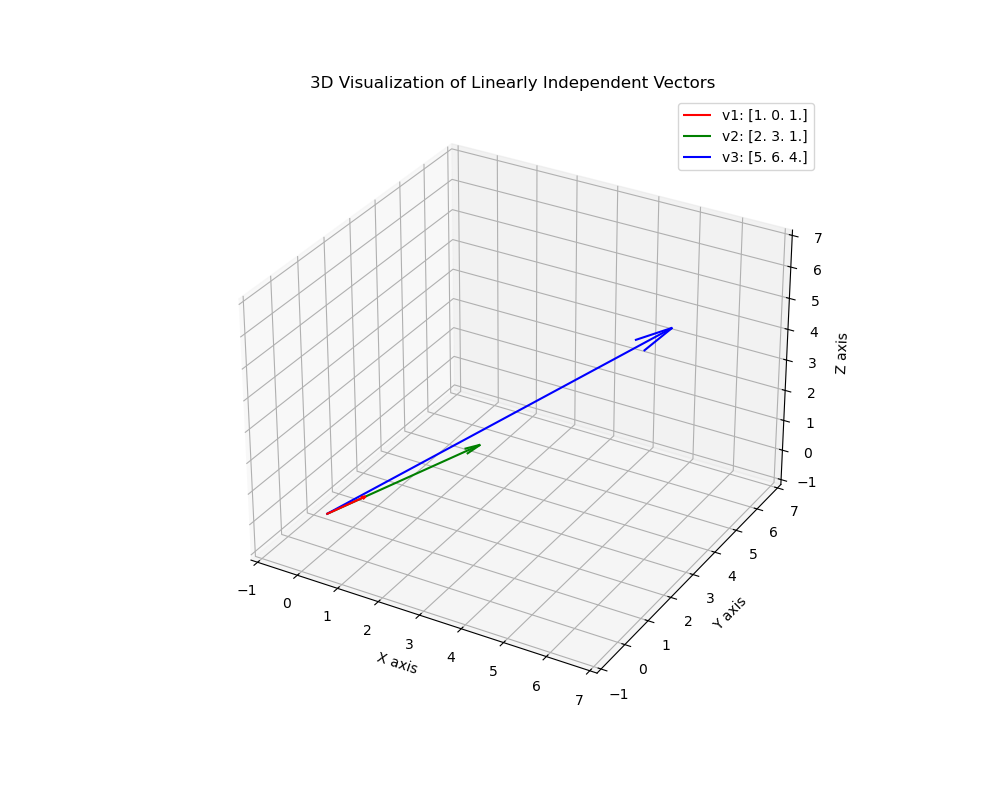
\includegraphics[width=\columnwidth, height=0.8\textheight, keepaspectratio]{figs/figure1.png}
        \end{center}
    \end{frame}
   

\end{document}
